\chapter{The model}

\subsection{Base package}

The diagram on figure \ref{model1} represent the first part of the package. In this diagram we can see the base of the game, there are the stone, the group that represent group of stone, coordinate of the stone and the color. All classes are the base of the game. 

The class group containt simple management of the collection it own and a special feature to melt group together. The method works simply, it take the groupe the bigger and transfert all the stone in this group and it add the liberty of the smallest group in the bigest, and set the group of all the stone to the biggest, and it return the final group.

  \begin{figure}[h!]
  \centering
  \scalebox{0.5}{
      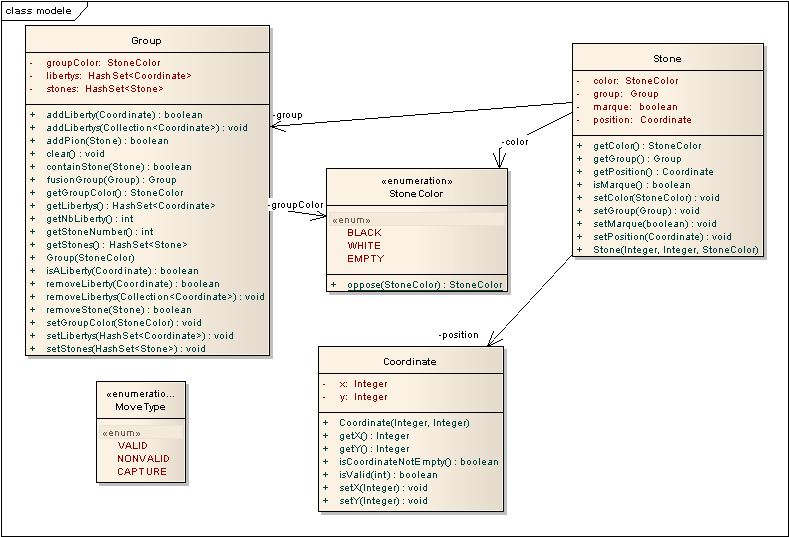
\includegraphics{image/model_class_diagram_part1.png}
  }
  \caption{Model package part1}
\label{model1} 
 \end{figure}

The diagram on figure \ref{model2} represent the second part of the package. In this diagram we can see the "heart" of the game, it containt the actual board and all the method to add stone, it manage the game's rules. All this process is manage by the goban class. 

The Gamehandler is kind of the model manager, it manage the AI, the board, if the ai is activate and a move play by the player, the gamehandler will tell to the AI to play. It check if there is a winner.

The goban class is the board and all the method relative to the game evolution. It containt method to add stone, to remove stone, to handle capture, to check if a move is allowed, etc. 

To check if a move is allowed, it check if there not a stone already on the slot, it check if there is liberty for the stone, but if there no liberty for the stone but remove the last liberty of an enemy group, the move is allowed.

The goban class offer other utility method like get the liberty list of a stone, the neighbors of a stone.

This class handle two mode of game evolution, one that remove stone on the board if there a capture and a one that don't remove stone, the second one is used by the AI to prepare move and see if it capture stone. This last mode is use with the removeStone method that reform the group(by backtraking the stone formation's), it works better is the game is not corrupted by the AI move.

  \begin{figure}[h!]
  \centering
  \scalebox{0.5}{
      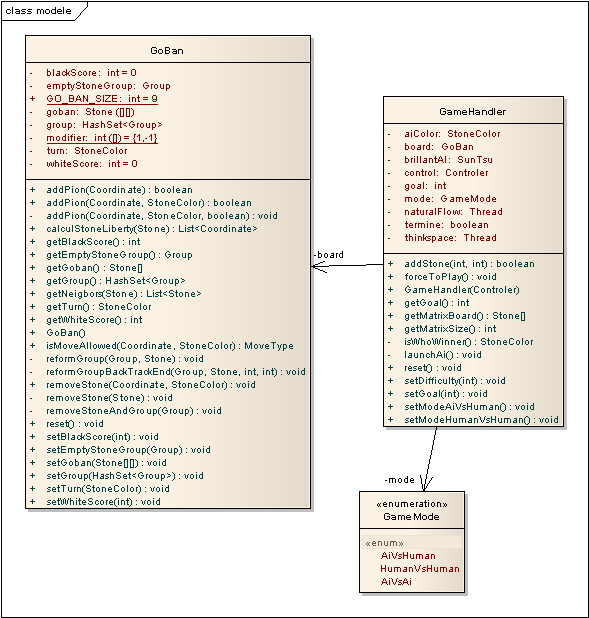
\includegraphics{image/model_class_diagram_part2.png}
  }
  \caption{Model package part2}
\label{model2} 
 \end{figure}


\subsection{Intelligence package}

The diagram on figure \ref{intel} represent the sub package inteligence. In this diagram we can see the "brain" of the game, our brillant(or not) AI with a awesome name. This package contain all the class used by the AI to calculate the "best" move. 

The algorithm to calculate the best move is basically the AlphaBeta algorithm, but every intermediary result is store for the case of an interruption of the calculation. 

To have the possibility of interrupt the calculation, the calculation is launch in a new thread by the gameHandler class, and after another thread wait for the result, it use the wait() method, then when the calculation is over, the thread who wait the result is notify() that is not have to wait more time. To interrupt the calculation it just have to notify() and then the result thread will get an intermediary result.


  \begin{figure}[h!]
  \centering
  \scalebox{0.6}{
      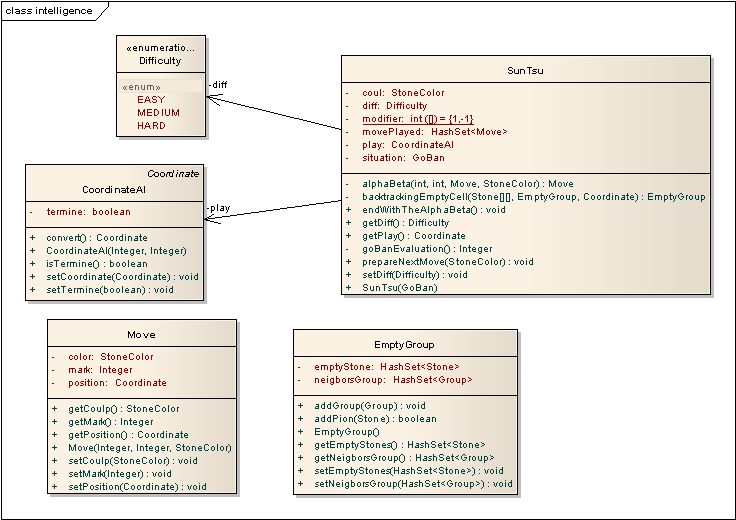
\includegraphics{image/model_intelligence_class_diagram.png}
  }
  \caption{Intelligence sub package}
\label{intel} 
 \end{figure}

The evaluation of a situation is made by the SunTsu class, it check the liberty of all groups, it check if there some eyes in the game by backtracking groups of empty cells, if there so surround by one group it is an eye.


\clearpage
